\documentclass[10pt]{article}
\usepackage[utf8]{inputenc}
\usepackage[T1]{fontenc}
\usepackage{amsmath}
\usepackage{amsfonts}
\usepackage{amssymb}
\usepackage[version=4]{mhchem}
\usepackage{stmaryrd}
\usepackage{bbold}
\usepackage{graphicx}
\usepackage[export]{adjustbox}
\graphicspath{ {./images/} }

\begin{document}
\section*{MATHEMATICS}
\section*{SECTION-A}
\begin{enumerate}
  \setcounter{enumi}{60}
  \item The domain of \(f(x)=\frac{\log _{(x+1)}(x-2)}{e^{2 \log _{e} x}-(2 x+3)}, x \in R\) is\\
(1) \(\mathbb{R}-\{1-3\}\)\\
(2) \((2, \infty)-\{3\}\)\\
(3) \((-1, \infty)-\{3\}\)\\
(4) \(\mathbb{R}-\{3\}\)
\end{enumerate}

Official Ans. by NTA (2)\\
Allen Ans. (2)\\
Sol. \(x-2>0 \Rightarrow x>2\)\\
\(\mathrm{x}+1>0 \Rightarrow \mathrm{x}>-1\)\\
\(x+1 \neq 1 \Rightarrow x \neq 0\) and \(x>0\)\\
Denominator\\
\(x^{2}-2 x-3 \neq 0\)\\
\((x-3)(x+1) \neq 0\)\\
\(x \neq-1,3\)\\
So Ans \((2, \infty)-\{3\}\)\\
62. Let \(\mathrm{f}: \mathrm{R} \rightarrow \mathrm{R}\) be a function such that \(f(x)=\frac{x^{2}+2 x+1}{x^{2}+1}\). Then\\
(1) \(f(x)\) is many-one in \((-\infty,-1)\)\\
(2) \(f(x)\) is many-one in \((1, \infty)\)\\
(3) \(f(x)\) is one-one in \([1, \infty)\) but not in \((-\infty, \infty)\)\\
(4) \(f(x)\) is one-one in \((-\infty, \infty)\)

Official Ans. by NTA (3)\\
Allen Ans. (3)

Sol.\\
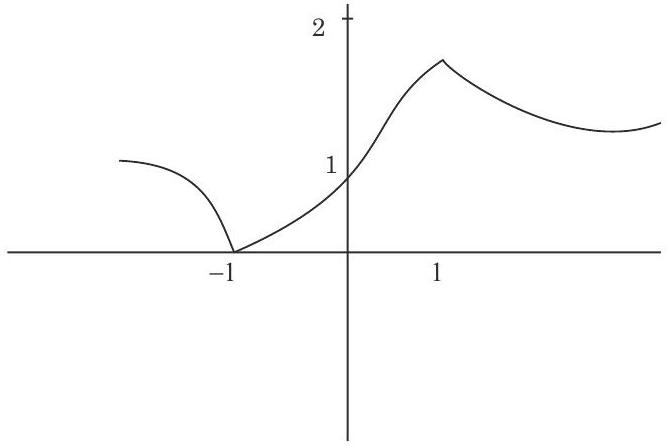
\includegraphics[max width=\textwidth, center]{2025_10_03_00eb3af2dfb61b7a2313g-01}

\[
\begin{aligned}
& f(x)=\frac{(x+1)^{2}}{x^{2}+1}=1+\frac{2 x}{x^{2}+1} \\
& f(x)=1+\frac{2}{x+\frac{1}{x}}
\end{aligned}
\]

\section*{TEST PAPER WITH SOLUTION}
\begin{enumerate}
  \setcounter{enumi}{62}
  \item For two non-zero complex number \(z_{1}\) and \(z_{2}\), if \(\operatorname{Re}\left(z_{1} z_{2}\right)=0\) and \(\operatorname{Re}\left(z_{1}+z_{2}\right)=0\), then which of the following are possible ?\\
(A) \(\operatorname{Im}\left(\mathrm{z}_{1}\right)>0\) and \(\operatorname{Im}\left(\mathrm{z}_{2}\right)>0\)\\
(B) \(\operatorname{Im}\left(\mathrm{z}_{1}\right)<0\) and \(\operatorname{Im}\left(\mathrm{z}_{2}\right)>0\)\\
(C) \(\operatorname{Im}\left(\mathrm{z}_{1}\right)>0\) and \(\operatorname{Im}\left(\mathrm{z}_{2}\right)<0\)\\
(D) \(\operatorname{Im}\left(\mathrm{z}_{1}\right)<0\) and \(\operatorname{Im}\left(\mathrm{z}_{2}\right)<0\)
\end{enumerate}

Choose the correct answer from the options given below :\\
(1) B and D\\
(2) B and C\\
(3) A and B\\
(4) A and C

Official Ans. by NTA (2)\\
Allen Ans. (2)

Sol. \(z_{1}=x_{1}+i y_{1}\)\\
\(\mathrm{z}_{2}=\mathrm{x}_{2}+\mathrm{iy}_{2}\)\\
\(\operatorname{Re}\left(\mathrm{z}_{1} \mathrm{z}_{2}\right)=\mathrm{x}_{1} \mathrm{x}_{2}-\mathrm{y}_{1} \mathrm{y}_{2}=0\)\\
\(\operatorname{Re}\left(\mathrm{z}_{1}+\mathrm{z}_{2}\right)=\mathrm{x}_{1}+\mathrm{x}_{2}=0\)\\
\(x_{1} \& x_{2}\) are of opposite sign\\
\(y_{1} \& y_{2}\) are of opposite sign\\
64. Let \(\lambda \neq 0\) be a real number. Let \(\alpha, \beta\) be the roots of the equation \(14 x^{2}-3 l x+3 \lambda=0\) and \(\alpha, \gamma\) be the roots of the equation \(35 x^{2}-53 x+4 \lambda=0\). Then \(\frac{3 \alpha}{\beta}\) and \(\frac{4 \alpha}{\gamma}\) are the roots of the equation :\\
(1) \(7 \mathrm{x}^{2}+245 \mathrm{x}-250=0\)\\
(2) \(7 \mathrm{x}^{2}-245 \mathrm{x}+250=0\)\\
(3) \(49 x^{2}-245 x+250=0\)\\
(4) \(49 x^{2}+245 x+250=0\)

Official Ans. by NTA (3)\\
Allen Ans. (3)

Sol. \(\quad 14 \mathrm{x}^{2}-31 \mathrm{x}+3 \lambda=0\)

\[
\alpha+\beta=\frac{31}{14} \ldots .(1) \text { and } \alpha \beta=\frac{3 \lambda}{14}
\]

\(35 \mathrm{x}^{2}-53 \mathrm{x}+4 \lambda=0\)

\[
\alpha+\gamma=\frac{53}{35} \ldots .(3) \text { and } \alpha \gamma=\frac{4 \lambda}{35}
\]

\(\frac{(2)}{(4)} \Rightarrow \frac{\beta}{\gamma}=\frac{3 \times 35}{4 \times 14}=\frac{15}{8} \Rightarrow \beta=\frac{15}{8} \gamma\)\\
(1) - (3) \(\Rightarrow \beta-\gamma=\frac{31}{14}-\frac{53}{35}=\frac{155-106}{70}=\frac{7}{10}\)\\
\(\frac{15}{8} \gamma-\gamma=\frac{7}{10} \Rightarrow \gamma=\frac{4}{5}\)\\
\(\Rightarrow \beta=\frac{15}{8} \times \frac{4}{5}=\frac{3}{2}\)\\
\(\Rightarrow \alpha=\frac{31}{14}-\beta=\frac{31}{14}-\frac{3}{2}=\frac{5}{7}\)\\
\(\Rightarrow \lambda=\frac{14}{3} \alpha \beta=\frac{14}{3} \times \frac{5}{7} \times \frac{3}{2}=5\)\\
so, sum of roots \(\frac{3 \alpha}{\beta}+\frac{4 \alpha}{\gamma}=\left(\frac{3 \alpha \gamma+4 \alpha \beta}{\beta \gamma}\right)\)\\
\(=\frac{\left(3 \times \frac{4 \lambda}{35}+4 \times \frac{3 \lambda}{14}\right)}{\beta \gamma}=\frac{12 \lambda(14+35)}{14 \times 35 \beta \gamma}\)\\
\(=\frac{49 \times 12 \times 5}{490 \times \frac{3}{2} \times \frac{4}{5}}=5\)

Product of roots\\
\(=\frac{3 \alpha}{\beta} \times \frac{4 \alpha}{\gamma}=\frac{12 \alpha^{2}}{\beta \gamma}=\frac{12 \times \frac{25}{49}}{\frac{3}{2} \times \frac{4}{5}}=\frac{250}{49}\)

So, required equation is \(x^{2}-5 x+\frac{250}{49}=0\)\\
\(\Rightarrow 49 x^{2}-245 x+250=0\)\\
65. Consider the following system of questions\\
\(\alpha x+2 y+z=1\)\\
\(2 \alpha x+3 y+z=1\)\\
\(3 x+\alpha y+2 z=\beta\)\\
For some \(\alpha, \beta \in \mathbb{R}\). Then which of the following is NOT correct.\\
(1) It has no solution if \(\alpha=-1\) and \(\beta \neq 2\)\\
(2) It has no solution for \(\alpha=-1\) and for all \(\beta \in \mathbb{R}\)\\
(3) It has no solution for \(\alpha=3\) and for all \(\beta \neq 2\)\\
(4) It has a solution for all \(\alpha \neq-1\) and \(\beta=2\)

Official Ans. by NTA (2)\\
Allen Ans. (2)\\
Sol. \(\quad D=\left|\begin{array}{ccc}\alpha & 2 & 1 \\ 2 \alpha & 3 & 1 \\ 3 & \alpha & 2\end{array}\right|=0 \Rightarrow \alpha=-1,3\)\\
\(D_{x}=\left|\begin{array}{lll}2 & 1 & 1 \\ 3 & 1 & 1 \\ \alpha & 2 & \beta\end{array}\right|=0 \Rightarrow \beta=2\)\\
\(D_{y}=\left|\begin{array}{ccc}\alpha & 1 & 1 \\ 2 \alpha & 1 & 1 \\ 3 & 2 & \beta\end{array}\right|=0\)\\
\(D_{z}=\left|\begin{array}{ccc}\alpha & 2 & 1 \\ 2 \alpha & 3 & 1 \\ 3 & \alpha & \beta\end{array}\right|=0\)\\
\(\beta=2, \alpha=-1\)\\
\(\alpha=-1, \beta=2\) Infinite solution\\
66. Let \(\alpha\) and \(\beta\) be real numbers. Consider a \(3 \times 3\) matrix A such that \(\mathrm{A}^{2}=3 \mathrm{~A}+\alpha \mathrm{I}\). If \(\mathrm{A}^{4}=21 \mathrm{~A}+\beta \mathrm{I}\), then\\
(1) \(\alpha=1\)\\
(2) \(\alpha=4\)\\
(3) \(\beta=8\)\\
(4) \(\beta=-8\)

Official Ans. by NTA (4)\\
Allen Ans. (4)

Sol. \(A^{2}=3 A+\alpha I\)\\
\(\mathrm{A}^{3}=3 \mathrm{~A}^{2}+\alpha \mathrm{A}\)\\
\(\mathrm{A}^{3}=3(3 \mathrm{~A}+\alpha \mathrm{I})+\alpha \mathrm{A}\)\\
\(\mathrm{A}^{3}=9 \mathrm{~A}+\alpha \mathrm{A}+3 \alpha \mathrm{I}\)\\
\(\mathrm{A}^{4}=(9+\alpha) \mathrm{A}^{2}+3 \alpha \mathrm{~A}\)\\
\(=(9+\alpha)(3 \mathrm{~A}+\alpha \mathrm{I})+3 \alpha \mathrm{~A}\)\\
\(=\mathrm{A}(27+6 \alpha)+\alpha(9+\alpha)\)\\
\(\Rightarrow 27+6 \alpha=21 \Rightarrow \alpha=-1\)\\
\(\Rightarrow \beta=\alpha(9+\alpha)=-8\)\\
67. Let \(x=2\) be a root of the equation \(x^{2}+p x+q=0\)\\
and \(f(x)=\left\{\begin{array}{cc}\frac{1-\cos \left(x^{2}-4 p x+q^{2}+8 q+16\right)}{(x-2 p)^{4}}, & x \neq 2 p \\ 0, & x=2 p\end{array}\right.\)\\
Then \(\lim _{x \rightarrow 2 p^{+}}[f(x)]\)\\[0pt]
where [ . . ] denotes greatest integer function, is\\
(1) 2\\
(2) 1\\
(3) 0\\
(4) -1

Official Ans. by NTA (3)\\
Allen Ans. (3)\\
Sol.\\
\(\lim _{x \rightarrow 2 p^{+}}\left(\frac{1-\cos \left(x^{2}-4 p x+q^{2}+8 q+16\right)}{\left(x^{2}-4 p x+q^{2}+8 q+16\right)^{2}}\right)\left(\frac{\left(x^{2}-4 p x+q^{2}+8 q+16\right)^{2}}{(x-2 p)^{2}}\right)\)\\
\(\lim _{\mathrm{h} \rightarrow 0} \frac{1}{2}\left(\frac{(2 \mathrm{p}+\mathrm{h})^{2}-4 \mathrm{p}(2 \mathrm{p}+\mathrm{h})+\mathrm{q}^{2}+82+16}{\mathrm{~h}^{2}}\right)^{2}=\frac{1}{2}\)\\
Using L'Hospital's

\[
\lim _{x \rightarrow 2 p^{+}}[f(x)]=0
\]

\begin{enumerate}
  \setcounter{enumi}{67}
  \item Let \(f(x)=x+\frac{a}{\pi^{2}-4} \sin x+\frac{b}{\pi^{2}-4} \cos x\), \(x \in \mathbb{R} \quad\) be a function which satisfies \(f(x)=x+\int_{0}^{\pi / 2} \sin (x+y) f(y) d y\). Then \((\mathrm{a}+\mathrm{b})\) is equal to\\
(1) \(-\pi(\pi+2)\)\\
(2) \(-2 \pi(\pi+2)\)\\
(3) \(-2 \pi(\pi-2)\)\\
(4) \(-\pi(\pi-2)\)
\end{enumerate}

Official Ans. by NTA (2)\\
Allen Ans. (2)

Sol. \(f(x)=x+\int_{0}^{\pi / 2}(\sin x \cos y+\cos x \sin y) f(y) d y\)

\[
f(x)=x+\int_{0}^{\pi / 2}((\cos y f(y) d y) \sin x+(\sin y f(y) d y) \cos x)
\]

On comparing with\\
\(f(x)=x+\frac{a}{\pi^{2}-4} \sin x+\frac{b}{\pi^{2}-4} \cos x, x \in \mathbb{R}\) then

\[
\Rightarrow \frac{a}{\pi^{2}-4}=\int_{0}^{\pi / 2} \cos y f(y) d y
\]

\(\Rightarrow \frac{b}{\pi^{2}-4}=\int_{0}^{\pi / 2} \sin y f(y) d y\)

Add (2) and (3)

\[
\frac{a+b}{\pi^{2}-4}=\int_{0}^{\pi / 2}(\sin y+\cos y) f(y) d y
\]

\[
\frac{a+b}{\pi^{2}-4}=\int_{0}^{\pi / 2}(\sin y+\cos y) f\left(\frac{\pi}{2}-y\right) d y
\]

Add (4) and (5)

\[
\begin{aligned}
\frac{2(a+b)}{\pi^{2}-4} & =\int_{0}^{\pi / 2}(\sin y+\cos y)\left(\frac{\pi}{2}+\frac{(a+b)}{\pi^{2}-4}(\sin y+\cos y)\right) d y \\
& =\pi+\frac{a+b}{\pi^{2}-4}\left(\frac{\pi}{2}+1\right)
\end{aligned}
\]

\((a+b)=-2 \pi(\pi+2)\)\\
69. Let \(\mathrm{A}=\left\{(\mathrm{x}, \mathrm{y}) \in \mathbb{R}^{2}: \mathrm{y} \geq 0,2 \mathrm{x} \leq \mathrm{y} \leq \sqrt{4-(\mathrm{x}-1)^{2}}\right\}\) and \(\mathrm{B}=\left\{(\mathrm{x}, \mathrm{y}) \in \mathbb{R} \times \mathbb{R}: 0 \leq \mathrm{y} \leq \min \left\{2 \mathrm{x}, \sqrt{4-(\mathrm{x}-1)^{2}}\right\}\right\}\) Then the ratio of the area of A to the area of B is\\
(1) \(\frac{\pi-1}{\pi+1}\)\\
(2) \(\frac{\pi}{\pi-1}\)\\
(3) \(\frac{\pi}{\pi+1}\)\\
(4) \(\frac{\pi+1}{\pi-1}\)

Official Ans. by NTA (1)\\
Allen Ans. (1)

Sol. \(y^{2}+(x-1)^{2}=4\)\\
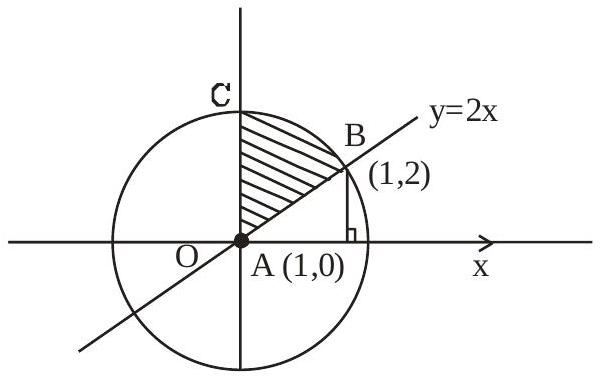
\includegraphics[max width=\textwidth, center]{2025_10_03_00eb3af2dfb61b7a2313g-04(1)}\\
shaded portion \(=\) circular \((\mathrm{OABC})\)\\
\(-\operatorname{Ar}(\Delta \mathrm{OAB})\)\\
\(=\frac{\pi(4)}{4}-\frac{1}{2}(2)(1)\)\\
\(\mathrm{A}=(\pi-1)\)\\
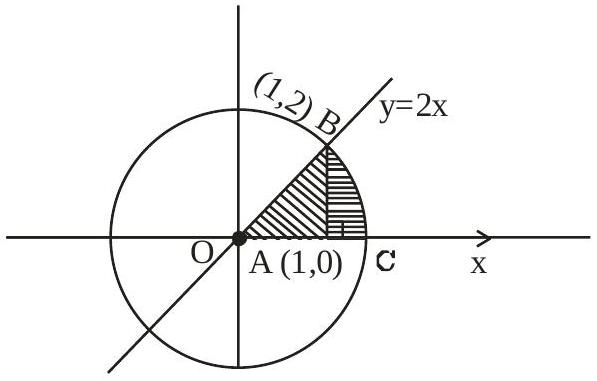
\includegraphics[max width=\textwidth, center]{2025_10_03_00eb3af2dfb61b7a2313g-04(2)}

Area \(B=\operatorname{Ar}(\triangle A O B)+\) Area of arc of circle \((A B C)\)\\
\(=\frac{1}{2}(1)(2)+\frac{\pi(2)^{2}}{4}=\pi+1\)\\
\(\frac{\mathrm{A}}{\mathrm{B}}=\frac{\pi-1}{\pi+1}\)\\
70. Let \(\Delta\) be the area of the region\\
\(\left\{(\mathrm{x}, \mathrm{y}) \in \mathbb{R}^{2}: \mathrm{x}^{2}+\mathrm{y}^{2} \leq 21, \mathrm{y}^{2} \leq 4 \mathrm{x}, \mathrm{x} \geq 1\right\} . \quad\) Then \(\frac{1}{2}\left(\Delta-21 \sin ^{-1} \frac{2}{\sqrt{7}}\right)\) is equal to\\
(1) \(2 \sqrt{3}-\frac{1}{3}\)\\
(2) \(\sqrt{3}-\frac{2}{3}\)\\
(3) \(2 \sqrt{3}-\frac{2}{3}\)\\
(4) \(\sqrt{3}-\frac{4}{3}\)

Official Ans. by NTA (4)\\
Allen Ans. (4)

Sol.\\
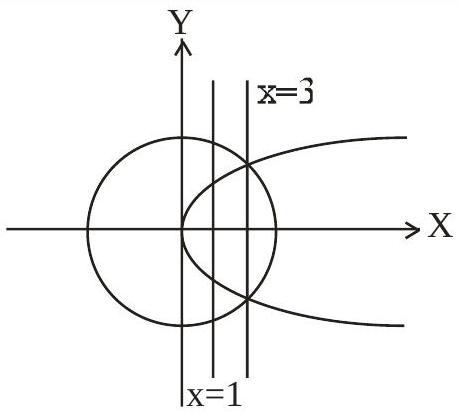
\includegraphics[max width=\textwidth, center]{2025_10_03_00eb3af2dfb61b7a2313g-04}

Area \(2 \int_{1}^{3} 2 \sqrt{x} d x+2 \int_{3}^{\sqrt{21}} \sqrt{21-x^{2} d x}\)\\
\(\Delta=\frac{8}{3}(3 \sqrt{3}-1)+21 \sin ^{-1}\left(\frac{2}{\sqrt{7}}\right)-6 \sqrt{3}\)\\
\(\frac{1}{2}\left(\Delta-21 \sin ^{-1}\left(\frac{2}{\sqrt{7}}\right)\right)=\frac{2 \sqrt{3}-\frac{8}{3}}{2}\)\\
\(=\sqrt{3}-\frac{4}{3}\)\\
71. A light ray emits from the origin making an angle \(30^{\circ}\) with the positive x -axis. After getting reflected by the line \(\mathrm{x}+\mathrm{y}=1\), if this ray intersects x -axis at Q , then the abscissa of Q is\\
(1) \(\frac{2}{(\sqrt{3}-1)}\)\\
(2) \(\frac{2}{3+\sqrt{3}}\)\\
(3) \(\frac{2}{3-\sqrt{3}}\)\\
(4) \(\frac{\sqrt{3}}{2(\sqrt{3}+1)}\)

Official Ans. by NTA (2)\\
Allen Ans. (2)\\
Sol. Slope of reflected ray \(=\tan 60^{\circ}=\sqrt{3}\)

Line \(\mathrm{y}=\frac{\mathrm{x}}{\sqrt{3}}\) intersect \(\mathrm{y}+\mathrm{x}=1\) at \(\left(\frac{\sqrt{3}}{\sqrt{3}+1}, \frac{1}{\sqrt{3}+1}\right)\)

Equation of reflected ray is\\
\(y-\frac{1}{\sqrt{3}+1}=\sqrt{3}\left(x-\frac{\sqrt{3}}{\sqrt{3}+1}\right)\)

Put \(y=0 \Rightarrow x=\frac{2}{3+\sqrt{3}}\)\\
72. Let B and C be the two points on the line \(\mathrm{y}+\mathrm{x}=0\) such that B and C are symmetric with respect to the origin. Suppose A is a point on \(\mathrm{y}-2 \mathrm{x}=2\) such that \(\triangle \mathrm{ABC}\) is an equilateral triangle. Then, the area of the \(\triangle \mathrm{ABC}\) is\\
(1) \(3 \sqrt{3}\)\\
(2) \(2 \sqrt{3}\)\\
(3) \(\frac{8}{\sqrt{3}}\)\\
(4) \(\frac{10}{\sqrt{3}}\)

\section*{Official Ans. by NTA (3)}
Allen Ans. (3)

Sol.\\
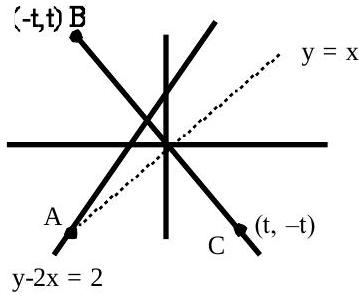
\includegraphics[max width=\textwidth, center]{2025_10_03_00eb3af2dfb61b7a2313g-05}

At A \(x=y\)\\
\(Y-2 x=2\)\\
(-2, -2)

Height from line \(\mathrm{x}+\mathrm{y}=0\)\\
\(\mathrm{h}=\frac{4}{\sqrt{2}}\)

Area of \(\Delta=\frac{\sqrt{3}}{4} \frac{\mathrm{~h}^{2}}{\sin ^{2} 60}=\frac{8}{\sqrt{3}}\)\\
73. Let the tangents at the points \(\mathrm{A}(4,-11)\) and \(\mathrm{B}(8,-5)\) on the circle \(x^{2}+y^{2}-3 x+10 y-15=0\), intersect at the point C . Then the radius of the circle, whose centre is C and the line joining A and B is its tangent, is equal to\\
(1) \(\frac{3 \sqrt{3}}{4}\)\\
(2) \(2 \sqrt{13}\)\\
(3) \(\sqrt{13}\)\\
(4) \(\frac{2 \sqrt{13}}{3}\)

Official Ans. by NTA (4)\\
Allen Ans. (4)

Sol. Equation of tangent at \(\mathrm{A}(4,-11)\) on circle is

\[
\begin{aligned}
& \Rightarrow 4 x-11 y-3\left(\frac{x+4}{2}\right)+10\left(\frac{y-11}{2}\right)-15=0 \\
& \Rightarrow 5 x-12 y-152=0 \ldots .(1)
\end{aligned}
\]

Equation of tangent at \(\mathrm{B}(8,-5)\) on circle is

\[
\begin{aligned}
& \Rightarrow 8 x-5 y-3\left(\frac{x+8}{2}\right)+10\left(\frac{y-5}{2}\right)-15=0 \\
& \Rightarrow 13 x-104=0 \Rightarrow x=8
\end{aligned}
\]

put in (1) \(\Rightarrow y=\frac{28}{3}\)

\[
r=\left|\frac{3.8+\frac{2.28}{3}-34}{\sqrt{13}}\right|=\frac{2 \sqrt{13}}{3}
\]

\begin{enumerate}
  \setcounter{enumi}{73}
  \item Let \([\mathrm{x}]\) denote the greatest integer \(\leq \mathrm{x}\). Consider the function \(\mathrm{f}(\mathrm{x})=\max \left\{\mathrm{x}^{2}, 1+[\mathrm{x}]\right\}\). Then the value of the integral \(\int_{0}^{2} f(x) d x\) is :\\
(1) \(\frac{5+4 \sqrt{2}}{3}\)\\
(2) \(\frac{8+4 \sqrt{2}}{3}\)\\
(3) \(\frac{1+5 \sqrt{2}}{3}\)\\
(4) \(\frac{4+5 \sqrt{2}}{3}\)
\end{enumerate}

\section*{Official Ans. by NTA (1) \\
 Allen Ans. (1)}
Sol.\\
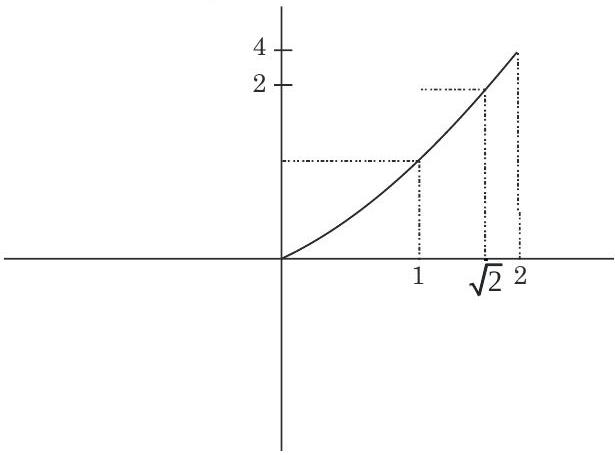
\includegraphics[max width=\textwidth, center]{2025_10_03_00eb3af2dfb61b7a2313g-05(1)}

\[
\begin{aligned}
& A=\int_{0}^{1} 1 \cdot d x+\int_{1}^{\sqrt{2}} 2 d x+\int_{\sqrt{2}}^{2} x^{2} d x \\
& =1+2 \sqrt{2}-2+\frac{8}{3}-\frac{2 \sqrt{2}}{3} \\
& =\frac{5}{3}+\frac{4 \sqrt{2}}{3}
\end{aligned}
\]

\begin{enumerate}
  \setcounter{enumi}{74}
  \item If the vectors \(\vec{a}=\lambda \hat{i}+\mu \hat{j}+4 \hat{k}, \vec{b}=2 \hat{i}+4 \hat{j}-2 \hat{k}\) and \(\vec{c}=2 \hat{i}+3 \hat{j}+\hat{k}\) are coplanar and the projection of \(\vec{a}\) on the vector \(\vec{b}\) is \(\sqrt{54}\) units, then the sum of all possible values of \(\lambda+\mu\) is equal to\\
(1) 0\\
(2) 6\\
(3) 24\\
(4) 18
\end{enumerate}

\section*{Official Ans. by NTA (3)}
\section*{Allen Ans. (3)}
Sol. \(\left|\begin{array}{ccc}\lambda & \mu & 4 \\ -2 & 4 & -2 \\ 2 & 3 & 1\end{array}\right|=0\)\\
\(\lambda(10)=\mu(2)+4(-14)=0\)\\
\(10 \lambda-2 \mu=56\)\\
\(5 \lambda-\mu=28\)\\
\(\frac{\overrightarrow{\mathrm{a}} \cdot \overrightarrow{\mathrm{b}}}{|\overrightarrow{\mathrm{b}}|}=\sqrt{54}\)\\
\(\frac{-2 \lambda+4 \mu-8}{\sqrt{24}}=\sqrt{54}\)\\
\(-2 \lambda+4 \mu-8=\sqrt{54 \times 24}\)

By solving equation (1) \& (2)\\
\(\Rightarrow \lambda+\mu=24\)\\
76. Fifteen football players of a club-team are given 15 T-shirts with their names written on the backside. If the players pick up the T-shirts randomly, then the probability that at least 3 players pick the correct T-shirt is\\
(1) \(\frac{5}{24}\)\\
(2) \(\frac{2}{15}\)\\
(3) \(\frac{1}{6}\)\\
(4) \(\frac{5}{36}\)

Official Ans. by NTA (3)\\
Allen Ans. (Bonus)\\
Sol.\\
Required probability \(=1-\frac{D_{(15)}+{ }^{15} C_{1} \cdot D_{(14)}+{ }^{15} C_{2} D_{(13)}}{15!}\)\\
Taking \(\mathrm{D}_{(15)}\) as \(\frac{15!}{e}\)\\
\(\mathrm{D}_{(14)}\) as \(\frac{14!}{e}\)\\
\(\mathrm{D}_{(13)}\) as \(\frac{13!}{e}\)

We get, \(1-\left(\frac{\frac{15!}{e}+15 \cdot \frac{14!}{e}+\frac{15 \times 14}{2} \times \frac{13!}{e}}{15!}\right)\)\\
\(=1-\left(\frac{1}{e}+\frac{1}{e}+\frac{1}{2 e}\right)=1-\frac{5}{2 e} \approx .08\)\\
77. Let \(f(\theta)=3\left(\sin ^{4}\left(\frac{3 \pi}{2}-\theta\right)+\sin ^{4}(3 \pi+\theta)\right)-2\left(1-\sin ^{2} 2 \theta\right)\) and \(S=\left\{\theta \in[0, \pi]: f^{\prime}(\theta)=-\frac{\sqrt{3}}{2}\right\}\). If \(4 \beta=\sum_{\theta \in S} \theta\), then \(f(\beta)\) is equal to\\
(1) \(\frac{11}{8}\)\\
(2) \(\frac{5}{4}\)\\
(3) \(\frac{9}{8}\)\\
(4) \(\frac{3}{2}\)

Official Ans. by NTA (2)\\
Allen Ans. (2)\\
Sol.\\
\(f(\theta)=3\left(\sin ^{4}\left(\frac{3 \pi}{2}-\theta\right)+\sin ^{4}(3 x+\theta)\right)-2\left(1-\sin ^{2} 2 \theta\right)\)\\
\(S=\left\{\theta \in[0, \pi]: f^{\prime}(\theta)=-\frac{\sqrt{3}}{2}\right\}\)\\
\(\Rightarrow \mathrm{f}(\theta)=3\left(\cos ^{4} \theta+\sin ^{4} \theta\right)-2 \cos ^{2} 2 \theta\)\\
\(\Rightarrow \mathrm{f}(\theta)=3\left(1-\frac{1}{2} \sin ^{2} 2 \theta\right)-2 \cos ^{2} 2 \theta\)\\
\(\Rightarrow \mathrm{f}(\theta)=3-\frac{3}{2} \sin ^{2} 2 \theta-2 \cos ^{2} \theta\)

\[
=\frac{3}{2}-\frac{1}{2} \cos ^{2} 2 \theta=\frac{3}{2}-\frac{1}{2}\left(\frac{1+\cos 4 \theta}{2}\right)
\]

\(f(\theta)=\frac{5}{4}-\frac{\cos 4 \theta}{4}\)\\
\(\mathrm{f}^{\prime}(\theta)=\sin 4 \theta\)\\
\(\Rightarrow \mathrm{f}^{\prime}(\theta)=\sin 4 \theta=-\frac{\sqrt{3}}{2}\)\\
\(\Rightarrow 4 \theta=\mathrm{n} \pi+(-1)^{\mathrm{n}} \frac{\pi}{3}\)\\
\(\Rightarrow \theta=\frac{\mathrm{n} \pi}{4}+(-1)^{\mathrm{n}} \frac{\pi}{12}\)

\[
\begin{aligned}
& \Rightarrow \theta=\frac{\pi}{12},\left(\frac{\pi}{4}-\frac{\pi}{12}\right),\left(\frac{\pi}{2}+\frac{\pi}{12}\right),\left(\frac{3 \pi}{4}-\frac{\pi}{12}\right) \\
& \Rightarrow 4 \beta=\frac{\pi}{4}+\frac{\pi}{2}+\frac{3 \pi}{4}=\frac{3 \pi}{2} \\
& \Rightarrow \beta=\frac{3 \pi}{8} \Rightarrow f(\beta)=\frac{5}{4}-\frac{\cos \frac{3 \pi}{2}}{4}=\frac{5}{4}
\end{aligned}
\]

\begin{enumerate}
  \setcounter{enumi}{77}
  \item If \(p, q\) and \(r\) are three propositions, then which of the following combination of truth values of \(\mathrm{p}, \mathrm{q}\) and \(r\) makes the logical expression \(\{(p \vee q) \wedge((\sim p) \vee r)\} \rightarrow((\sim q) \vee r)\) false ?\\
(1) \(p=T, q=F, r=T\)\\
(2) \(p=T, q=T, r=F\)\\
(3) \(p=F, q=T, r=F\)\\
(4) \(p=T, q=F, r=F\)
\end{enumerate}

Official Ans. by NTA (3)\\
Allen Ans. (3)\\
Sol.

\begin{center}
\begin{tabular}{|c|c|c|c|c|c|}
\hline
 & p & q & r & \((\mathrm{p} \vee \mathrm{q}) \wedge((\sim \mathrm{p}) \vee \mathrm{r})\) & \(\sim \mathrm{q} \vee \mathrm{r}\) \\
\hline
\((1)\) & T & F & T & T & T \\
\hline
\((2)\) & T & T & F & F & F \\
\hline
\((3)\) & F & T & F & T & F \\
\hline
\((4)\) & T & F & F & F & T \\
\hline
\end{tabular}
\end{center}

Option (3) \((\mathrm{p} \vee \mathrm{q}) \wedge(\sim \mathrm{q} \vee \mathrm{r}) \rightarrow(\sim \mathrm{p} \vee \mathrm{r})\) will be False.\\
79. There rotten apples are mixed accidently with seven good apples and four apples are drawn one by one without replacement. Let the random variable X denote the number of rotten apples. If \(\mu\) and \(\sigma^{2}\) represent mean and variance of \(X\), respectively, then \(10\left(\mu^{2}+\sigma^{2}\right)\) is equal to\\
(1) 20\\
(2) 250\\
(3) 25\\
(4) 30

Official Ans. by NTA (1)\\
Allen Ans. (1)

Sol.

\begin{center}
\begin{tabular}{|l|l|l|l|}
\hline
\(X\) & \(P(x)\) & \(X P(X)\) & \(X^{2} P(X)\) \\
\hline
0 & \(1 / 6\) & 0 & 0 \\
\hline
1 & \(1 / 2\) & \(1 / 2\) & \(1 / 2\) \\
\hline
2 & \(3 / 10\) & \(6 / 10\) & \(12 / 10\) \\
\hline
3 & \(1 / 30\) & \(1 / 10\) & \(9 / 30\) \\
\hline
\end{tabular}
\end{center}

\(\sum \mathrm{xP}(\mathrm{x})=\frac{6}{2}=\mu\)\\
\(\sigma^{2}=\sum \mathrm{x}^{2} \mathrm{P}(\mathrm{x})-\mu^{2}\)\\
\(\sigma^{2}+\mu^{2}=0+\frac{1}{2}+\frac{12}{10}+\frac{9}{30}=2\)\\
\(10\left(\sigma^{2}+\mu^{2}\right)=20\) Ans.\\
80. Let \(y=f(x)\) be the solution of the differential equation \(y(x+1) d x-x^{2} d y=0, y(1)=e\). Then \(\lim _{x \rightarrow 0^{+}} f(x)\) is equal to\\
(1) 0\\
(2) \(\frac{1}{e}\)\\
(3) \(e^{2}\)\\
(4) \(\frac{1}{e^{2}}\)

Official Ans. by NTA (1)\\
Allen Ans. (1)\\
Sol. \(\frac{x+1}{x^{2}} d x=\frac{d y}{y}\)\\
\(\ln x-\frac{1}{x}=\ln y+c\)\\
\((1, \mathrm{e})\)\\
\(\mathrm{c}=-2\)\\
\(\ln x-\frac{1}{x}=\ln y-2\)\\
\(y=e^{\ln x}-\frac{1}{x}+2\)\\
\(\lim _{x \rightarrow 0^{+}} e^{\ln x-1}-\frac{1}{x}+2\)\\
\(=e^{-\infty}\)\\
\(=0\)

\section*{SECTION-B}
\begin{enumerate}
  \setcounter{enumi}{80}
  \item Let the co-ordinates of one vertex of \(\triangle \mathrm{ABC}\) be \(\mathrm{A}(0,2, \alpha)\) and the other two vertices lie on the line \(\frac{x+\alpha}{5}=\frac{y-1}{2}=\frac{z+4}{3}\). For \(\alpha \in \mathbb{Z}\), if the area of \(\triangle \mathrm{ABC}\) is 21 sq. units and the line segment BC has length \(2 \sqrt{21}\) units, then \(\alpha^{2}\) is equal to \(\_\_\_\_\) .
\end{enumerate}

\section*{Official Ans. by NTA (9)}
\section*{Allen Ans. (9)}
Sol. A. \(\left(\mathrm{O}_{1} 2, \alpha\right)\)\\
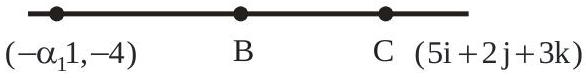
\includegraphics[max width=\textwidth, center]{2025_10_03_00eb3af2dfb61b7a2313g-08}

\[
\left|\frac{1}{2} \cdot 2 \sqrt{21} \cdot\right| \begin{array}{ccc}
\mathrm{i} & \mathrm{j} & \mathrm{k} \\
\alpha & 1 & \alpha+4 \\
5 & 2 & 3
\end{array}\left|\frac{1}{\sqrt{25+4+9}}\right|=21 \sqrt{21}
\]

\(\sqrt{(2 \alpha+5)^{2}+(2 \alpha+20)^{2}+(2 \alpha-5)^{2}}=\sqrt{21} \sqrt{38}\)\\
\(\Rightarrow 12 \alpha^{2}+80 \alpha+450=798\)\\
\(\Rightarrow 12 \alpha^{2}+80 \alpha-348=0\)\\
\(\Rightarrow \alpha=3 \Rightarrow \alpha^{2}=9\)\\
82. Let the equation of the plane P containing the line \(\mathrm{x}+10=\frac{8-\mathrm{y}}{2}=\mathrm{z}\) be \(\mathrm{ax}+\mathrm{by}+3 \mathrm{z}=2(\mathrm{a}+\mathrm{b})\) and the distance of the plane P from the point \((1,27,7)\) be c. Then \(a^{2}+b^{2}+c^{2}\) is equal to \(\_\_\_\_\) .

\section*{Official Ans. by NTA (355)}
\section*{Allen Ans. (355)}
Sol. The line \(\frac{x+10}{1}=\frac{y-8}{-2}=\frac{z}{1}\) have a point \((-10,8,0)\) with d. r. (1, -2, 1)\\
\(\because\) the plane \(\mathrm{ax}+\) by \(+3 \mathrm{z}=2(\mathrm{a}+\mathrm{b})\)\\
\(\Rightarrow \mathrm{b}=2 \mathrm{a}\)\\
\& dot product of d.r.'s is zero\\
\(\therefore \mathrm{a}-2 \mathrm{~b}+3=0\)\\
\(\therefore \mathrm{a}=1 \& \mathrm{~b}=2\)\\
Distance from ( \(1,27,7\) ) is\\
\(c=\frac{1+54+21-6}{\sqrt{14}}=\frac{70}{\sqrt{14}}=5 \sqrt{14}\)\\
\(\therefore \mathrm{a}^{2}+\mathrm{b}^{2}+\mathrm{c}^{2}=1+4+350\)\\
= 355\\
83. Suppose f is a function satisfying \(\mathrm{f}(\mathrm{x}+\mathrm{y})=\mathrm{f}(\mathrm{x})+\mathrm{f}(\mathrm{y})\) for all \(\quad x, y \in \mathbb{N} \quad\) and \(\quad f(1)=\frac{1}{5} . \quad\) If \(\sum_{n=1}^{m} \frac{f(n)}{n(n+1)(n+2)}=\frac{1}{12}\), then \(m\) is equal to \(\_\_\_\_\) .

Official Ans. by NTA (10)\\
Allen Ans. (10)\\
Sol. \(\because f(1)=\frac{1}{5} \therefore f(2)=f(1)+f(1)=\frac{2}{5}\)\\
\(f(2)=\frac{2}{5} \quad f(3)=f(2)+f(1)=\frac{3}{5}\)\\
\(f(3)=\frac{3}{5}\)\\
\(\therefore \sum_{n=1}^{m} \frac{f(n)}{n(n+1)(n+2)}\)\\
\(=\frac{1}{5} \sum_{n=1}^{m}\left(\frac{1}{n+1}-\frac{1}{n+2}\right)\)\\
\(=\frac{1}{5}\left(\frac{1}{2}-\frac{1}{3}+\frac{1}{3}-\frac{1}{4}+\ldots .+\frac{1}{m+1}-\frac{1}{m+2}\right)\)\\
\(=\frac{1}{5}\left(\frac{1}{2}-\frac{1}{m+2}\right)=\frac{m}{10(m+2)}=\frac{1}{12}\)\\
\(\therefore m=10\)\\
84. Let \(\mathrm{a}_{1}, \mathrm{a}_{2}, \mathrm{a}_{3}, \ldots\). be a GP of increasing positive numbers. If the product of fourth and sixth terms is 9 and the sum of fifth and seventh terms is 24 , then \(\mathrm{a}_{1} \mathrm{a}_{9}+\mathrm{a}_{2} \mathrm{a}_{4} \mathrm{a}_{9}+\mathrm{a}_{5}+\mathrm{a}_{7}\) is equal to \(\_\_\_\_\) .

Official Ans. by NTA (60)\\
Allen Ans. (60)\\
Sol. \(\mathrm{a}_{4} \cdot \mathrm{a}_{6}=9 \Rightarrow\left(\mathrm{a}_{5}\right)^{2}=9 \Rightarrow \mathrm{a}_{5}=3\)\\
\(\& a_{5}+a_{7}=24 \Rightarrow a_{5}+a_{5} r^{2}=24 \Rightarrow\left(1+r^{2}\right)=8 \Rightarrow r=\sqrt{7}\)\\
\(\Rightarrow \mathrm{a}=\frac{3}{49}\)\\
\(\Rightarrow a_{1} a_{9}+a_{2} a_{4} a_{9}+a_{5}+a_{7}=9+27+3+21=60\)\\
85. Let \(\vec{a}, \vec{b}\) and \(\vec{c}\) be three non-zero non-coplanar vectors. Let the position vectors of four points A , \(B, \quad C \quad\) and \(D \quad\) be \(\quad \vec{a}-\vec{b}+\vec{c}, \quad \lambda \vec{a}-3 \vec{b}+4 \vec{c}\), \(-\vec{a}+2 \vec{b}-3 \vec{c}\) and \(2 \vec{a}-4 \vec{b}+6 \vec{c}\) respectively. If \(\overrightarrow{A B}\), \(\overrightarrow{\mathrm{AC}}\) and \(\overrightarrow{\mathrm{AD}}\) are coplanar, then \(\lambda\) is :

Official Ans. by NTA (2)\\
Allen Ans. (2)\\
Sol. \(\overline{A B}=(\lambda-1) \bar{a}-2 \bar{b}+3 \bar{c}\)\\
\(\overline{A C}=2 \bar{a}+3 \bar{b}-4 \bar{c}\)\\
\(\overline{A D}=\bar{a}-3 \bar{b}+5 \bar{c}\)\\
\(\left|\begin{array}{ccc}\lambda-1 & -2 & 3 \\ -2 & 3 & -4 \\ 1 & -3 & 5\end{array}\right|=0\)\\
\(\Rightarrow(\lambda-1)(15-12)+2(-10+4)+3(6-3)=0\)\\
\(\Rightarrow(\lambda-1)=1 \Rightarrow \lambda=2\)\\
86. If all the six digit numbers \(\mathrm{x}_{1} \mathrm{x}_{2} \mathrm{x}_{3} \mathrm{x}_{4} \mathrm{x}_{5} \mathrm{x}_{6}\) with \(0<\mathrm{x}_{1}<\mathrm{x}_{2}<\mathrm{x}_{3}<\mathrm{x}_{4}<\mathrm{x}_{5}<\mathrm{x}_{6}\) are arranged in the increasing order, then the sum of the digits in the \(72^{\text {th }}\) number is \(\_\_\_\_\) .\\
Official Ans. by NTA (32)\\
Allen Ans. (32)\\
Sol.

\begin{center}
\begin{tabular}{|l|l|l|l|l|l|}
\hline
1 & 2 &  &  &  & \(={ }^{7} \mathrm{C}_{4}=35\) \\
\hline
1 & 3 &  &  &  & \(={ }^{6} \mathrm{C}_{4}=15\) \\
\hline
1 & 4 &  &  &  & \(={ }^{5} \mathrm{C}_{4}=5\) \\
\hline
1 & 5 &  &  &  & \(={ }^{4} \mathrm{C}_{4}=1\) \\
\hline
2 & 3 &  &  &  & \(={ }^{6} \mathrm{C}_{4}=15\) \\
\hline
\end{tabular}
\end{center}

\(245678 \rightarrow 72^{\text {th }}\) word\\
\(2+4+5+6+7+8=32\)\\
87. Let \(\mathrm{f}: \mathbb{R} \rightarrow \mathbb{R}\) be a differentiable function that satisfies the relation \(\mathrm{f}(\mathrm{x}+\mathrm{y})=\mathrm{f}(\mathrm{x})+\mathrm{f}(\mathrm{y})-1, \quad \forall \mathrm{x}\), \(y \in \mathbb{R}\). If \(\mathrm{f}^{\prime}(0)=2\), then \(|\mathrm{f}(-2)|\) is equal to \(\_\_\_\_\) .

Official Ans. by NTA (3)\\
Allen Ans. (3)

Sol. \(\mathrm{f}(\mathrm{x}+\mathrm{y})=\mathrm{f}(\mathrm{x})+\mathrm{f}(\mathrm{y})-1\)\\
\(f^{\prime}(x)=\lim _{h \rightarrow 0} \frac{f(x+h)-f(x)}{h}\)\\
\(f^{\prime}(x)=\lim _{h \rightarrow 0} \frac{f(h)-f(0)}{h}=f^{\prime}(0)=2\)\\
\(f^{\prime}(x)=2 \Rightarrow d y=2 d x\)\\
\(y=2 x+C\)\\
\(\mathrm{x}=0, \mathrm{y}=1, \mathrm{c}=1\)\\
\(\mathrm{y}=2 \mathrm{x}+1\)\\
\(|f(-2)|=|-4+1|=|-3|=3\)\\
88. If the co-efficient of \(x^{9}\) in \(\left(\alpha x^{3}+\frac{1}{\beta x}\right)^{11}\) and the co-efficient of \(x^{-9}\) in \(\left(\alpha x-\frac{1}{\beta x^{3}}\right)^{11}\) are equal, then \((\alpha \beta)^{2}\) is equal to \(\_\_\_\_\) .

Official Ans. by NTA (1)\\
Allen Ans. (1)\\
Sol. Coefficient of \(\mathrm{x}^{9}\) in \(\left(\alpha x^{3}+\frac{1}{\beta x}\right)={ }^{11} C_{6} \cdot \frac{\alpha^{5}}{\beta^{6}}\)\\
\(\because\) Both are equal\\
\(\therefore \frac{11}{C_{6}} \cdot \frac{\alpha^{5}}{\beta^{6}}=-\frac{11}{C_{5}} \cdot \frac{\alpha^{6}}{\beta^{5}}\)\\
\(\Rightarrow \frac{1}{\beta}=-\alpha\)\\
\(\Rightarrow \alpha \beta=-1\)\\
\(\Rightarrow(\alpha \beta)^{2}=1\)\\
89. Let the coefficients of three consecutive terms in the binomial expansion of \((1+2 \mathrm{x})^{\mathrm{n}}\) be in the ratio \(2: 5: 8\). Then the coefficient of the term, which is in the middle of these three terms, is \(\_\_\_\_\) .\\
Official Ans. by NTA (1120)\\
Allen Ans. (1120)

Sol. \(\mathrm{t}_{\mathrm{r}+1}={ }^{\mathrm{n}} \mathrm{C}_{\mathrm{r}}(2 \mathrm{x})^{\mathrm{r}}\)\\
\(\Rightarrow \frac{{ }^{n} C_{r-1}(2)^{r-1}}{{ }^{n} C_{r}(2)^{r}}=\frac{2}{5}\)\\
\(\Rightarrow \frac{\frac{n!}{(r-1)!(n-r+1)!}}{\frac{n!(2)}{r!(n-r)!}}=\frac{2}{5}\)\\
\(\Rightarrow \frac{\mathrm{r}}{\mathrm{n}-\mathrm{r}+1}=\frac{4}{5} \Rightarrow 5 \mathrm{r}=4 \mathrm{n}-4 \mathrm{r}+4\)\\
\(\Rightarrow 9 \mathrm{r}=4(\mathrm{n}+1)\)\\
\(\Rightarrow \frac{{ }^{n} C_{r}(2)^{r}}{{ }^{n} C_{r+1}(2)^{r+1}}=\frac{5}{8}\)\\
\(\Rightarrow \frac{\frac{n!}{r!(n-r)!}}{\frac{n!}{(r+1)!(n-r-1)!}}=\frac{5}{4} \Rightarrow \frac{r+1}{n-r}=\frac{5}{4}\)\\
\(\Rightarrow 4 \mathrm{r}+4=5 \mathrm{n}-5 \mathrm{r} \Rightarrow 5 \mathrm{n}-4=9 \mathrm{r}\)

From (1) and (2)\\
\(\Rightarrow 4 \mathrm{n}+4=5 \mathrm{n}-4 \Rightarrow \mathrm{n}=8\)\\
(1) \(\Rightarrow \mathrm{r}=4\)\\
so, coefficient of middle term is\\
\({ }^{8} \mathrm{C}_{4} 2^{4}=16 \times \frac{8 \times 7 \times 6 \times 5}{4 \times 3 \times 2 \times 1}=16 \times 70=1120\)\\
90. Five digit numbers are formed using the digits 1, 2, 3, 5, 7 with repetitions and are written in descending order with serial numbers. For example, the number 77777 has serial number 1. Then the serial number of 35337 is \(\_\_\_\_\) .

Official Ans. by NTA (1436)\\
Allen Ans. (1436)

Sol. No of 5 digit numbers starting with digit 1 \(=5 \times 5 \times 5 \times 5=625\)

No of 5 digit numbers starting with digit 2\\
\(=5 \times 5 \times 5 \times 5=625\)\\
No of 5 digit numbers starting with 31\\
\(=5 \times 5 \times 5=125\)\\
No of 5 digit numbers starting with 32\\
\(=5 \times 5 \times 5=125\)\\
No of 5 digit numbers starting with 33\\
\(=5 \times 5 \times 5=125\)\\
No of 5 digit numbers starting with 351\\
\(=5 \times 5=25\)\\
No of 5 digit numbers starting with 352\\
\(=5 \times 5=25\)\\
No of 5 digit numbers starting with 3531\\
\(=5\)\\
No of 5 digit numbers starting with 3532\\
\(=5\)\\
Before 35337 will be 4 numbers,\\
So rank of 35337 will be 1690

So, in descending order serial number will be\\
\(3125-1690+1=1436\)


\end{document}